\chapter{Protein thermodynamics}
{\hypersetup{linkcolor=GREYDARK}\minitoc}
\label{chap:intro-physic-proteins}

The previous chapters introduced codon models and methodology for estimating parameters of mutation, selection and drift from empirical data, but remained elusive on the nature of the fitness landscape underlying proteins and did not question the causal determining factor for the strength of selection.
This chapter will seek to clarify the relationship between phylogenetic codon models and biophysics of protein, such as to uncover the underlying properties of the selective pressures shaping protein-coding \acrshort{DNA} sequences.
Consequently, this chapter will present works at the interface between phylogenetic codon models and protein biophysics, where both fields are corroborated and consolidated by the other.
Within this interface, many questions arise regarding the compatibility and feedback between these fields.
Are the predictions of biophysical models of protein evolution compatible and confirmed by the application of phylogenetic codon models on empirical data?
Or the other way around, can phylogenetic codon models be informed by the underlying biophysics of proteins?
To answer such questions, the first section of this chapter will present the theoretical foundations of protein biophysics, focusing on protein stability imposed by structural constraints.
Subsequently, the second section will present how these models can explain in part the observed variation of selective constraints across genes, across sites and across branches observed with classical codon models.
Thirdly, moving from classical to mechanistic codon model, the next section will discuss how fitness landscapes estimated by mechanistic codon models can also be related to the underlying protein biophysics.
Finally, phylogenetic models augmented and incorporating the underlying biophysics are presented and the implication of such models is discussed.

Several authors have adequately reviewed the interface between both fields from a broad perspective~\citep{Liberles2012,Serohijos2014,Sikosek2014,Arenas2015,Echave2017,Bastolla2017}. This chapter, being aimed at evolutionary biologists familiar with phylogenetic codon models (already presented in chapter~\ref{chap:intro-codon-models}), addresses more specifically how such models fit within the prediction of protein biophysics.

% Also Sikosek T, Chan HS. 2014. Biophysics of protein evolution and evolutionary protein biophysics. J. R. Soc. Interface 11:20140419
\section{The link between protein biophysics and molecular evolution}
\label{sec:intro-protein-biophysics}

The ability of a protein to perform its function depends on the stability of its 3-dimensional folding structure, but also on its ability to bind ligands and/or interact with other proteins, both in terms of kinetics and stability.
Theoretically, thermodynamics and kinetics of proteins are expected to be related to their function, and hence to selective constraints~\citep{Bastolla2017}.

\subsection{Conformational stability of proteins}

In thermodynamics, the stability of a protein is determined by the Gibbs free energy of its folded conformation, in comparison to the free energy of its possible unfolded conformations.
Similarly to the mutation-selection Markov process defined in chapter~\ref{chap:intro-formalism}, it is possible to derive the equilibrium distribution of conformations, where fitness is analogous to the opposite of free energy (less energetic conformations are more stable) and population size is analogous to inverse temperature.
As a result, the probability of observing a protein in its folded conformation, given by the Boltzmann equation, is proportional to the exponential of the free energy of its folded conformation ($\GFold$):
\begin{equation}
    \probaFold = \frac{\e^{-\GFold / kT}}{\mathcal{Z}},
\end{equation}
where $k$ is the Boltzmann constant and $T$ is temperature in Kelvin, $\mathcal{Z}$ is a normalizing constant summed over all possible conformations, also called the conformational {partition function}.
The conformational partition function is related to the free energy of the folded state and of all the possible unfolded states:
\begin{align}
    \mathcal{Z} & = \e^{-\GFold / kT} + \sum\limits_{\text{unfolded}} \e^{-\G_{\text{unfolded}} / kT} \\
    & = \e^{-\GFold / kT} + \e^{-\GUnfold / kT},
\end{align}
where $\GUnfold$ encompasses the free energy of all the possible unfolded conformations.
Altogether, the probability of observing the protein in folded conformation can then be re-expressed as:
\begin{align}
    \probaFold & = \frac{\e^{-\GFold / kT}}{\e^{-\GFold / kT} + \e^{-\GUnfold / kT}}, \\
    & = \frac{\e^{-\DeltaG/kT}}{ 1 + \e^{-\DeltaG/kT} }, \\
    & = \frac{1}{ 1 + \e^{\DeltaG/kT} }.
\end{align}
where $\DeltaG = \GFold - \GUnfold$.
Thus, in order for a protein to fold into its native state with high probability, the free energy gap ($\DeltaG$) has to be both negative and large in absolute value, as depicted in figure~\ref{fig:intro-proba-folding}.

\begin{figure}[H]
    \centering
    \includegraphics[width=0.8\textwidth, page=5] {figures.pdf}
    \caption[Probability of folding]{
    Probability of folding ($\probaFold$) as a function of the free energy gap ($\DeltaG = \GFold - \GUnfold$).
    $\DeltaG$ is in kcal/mol and $1/kT=1.686$ mol/kcal at room temperature.
    The free energy gap has to be both negative and large in absolute value for the protein to be folded.
    }
    \label{fig:intro-proba-folding}
\end{figure}

In this context, mutations of the proteins stabilize the protein only if they decrease the free energy of the folded conformations more than they decrease the free energy of unfolded conformations.
For example, a transition to an amino acid that decreases by the same amount the free energy of both folded and unfolded conformations will have no impact on the stability of the protein.
As a result, protein stability can be increased by stabilizing the folded conformation (positive design) or destabilizing the competing unfolded conformations (negative design).
We can thus characterize the destabilizing effect of a mutation by its:
\begin{equation}
    \EmpiricalDeltaDeltaG = \DeltaG \left( \text{Mutant} \right) - \DeltaG  \left( \text{Wild type} \right),
\end{equation}
where by definition $\EmpiricalDeltaDeltaG <0 $ for stabilizing mutations, and conversely $\EmpiricalDeltaDeltaG > 0 $ for destabilizing mutations.

Free energy gaps $\DeltaG$ can be experimentally measured, and fall within the range of $-25$ to $-5$ kcal/mol~\citep{Kumar2006, Gromiha2016}.
Moreover, empirical measurements of folding stability changes due to single point mutations can also be obtained experimentally. This process is costly and has to be done for each single mutation~\citep{Rocklin2017}.

Alternatively, the free energy gap of a protein can be computed with a biophysical model of the protein, by modelling the atomic structure and the potential energy of contact between residues at the atomic level in a 3-dimensional structure.
Computing the free energy gap for a given protein sequence is challenging for any given conformation of the backbone, since it also depends on the conformation of the side chains as well as the solvent (water).
To allow for faster computation, coarse-grained approximations have been proposed, in the form of statistical potentials, which approximate free energy ($G$) as a sum of free energy terms over all pairwise contacts between residues across the protein~\citep{Miyazawa1985}.

For a given folded conformation of the protein, the statistical potential gives $\GFold$.
However, in order to get $\DeltaG$, one still needs to sum over all unfolded conformations to compute $\mathcal{Z}$, or $\GUnfold$.
Models typically approximate the distribution of unfolded Gibbs free energy using representative decoy conformations for which energy is computed, assuming a quasi-chemical or normal approximation~\citep{Goldstein2011}.

Alternatively, in order to explicitly sum over all possible conformations, some models approximate the structure and dynamics of proteins by 2-dimensional lattice models with regular pavement~\citep{Taverna2002, Noivirt-Brik2009}.
Lattice models are designed to sum over all possible conformations, and are useful as a theoretical construct to gain new insights about biophysics and protein evolution.
However, lattice models are empirically less directly usable.
In between these two extremes, many models can approximate with various degrees of freedom and parametrization the relationship from sequence to stability.

\subsection{From stability to fitness}

Empirically, a large body of evidence indicates that the stability, or, in other words, the ability to fold in globular conformation, is a target of natural selection~\citep{Sikosek2014}.
Even though the association between protein sequence and protein stability is within reach and can be obtained with various degrees of approximations, the association between protein stability and fitness is more elusive and difficult to apprehend.
It is known that protein stability is related to fitness, as demonstrated by a study of beta-lactamase TEM-1 mutants~\citep{Jacquier2013}, or illustrated by the use of functional assays to identify stabilizing mutations~\citep{Araya2012}.
However, it is not clear whether protein stability increases fitness by being more efficient, or whether it is the deleterious cytotoxic effect of unfolded proteins that results in purifying selection for destabilizing mutations.
Additionally, the ability to bind other proteins may interfere with stability against misfolding, and large functional movements may imply a stability cost.

The relationship between stability and fitness raises the more general question of why proteins are marginally stable.
Indeed, the optimal stability is never achieved, and two types of explanation have been proposed.
Firstly, that it could be the consequence of the stability-activity trade-off such that proteins are selected for an intermediate stability.
Secondly, and more fundamentally, that it is an expectation of the mutation-selection equilibrium even under directional selection for stability~\citep{Taverna2002}.
These two explanations are not mutually incompatible, and can both explain the observed marginal stability of proteins.

Furthermore, translation errors act like point mutations, with a fairly high translation error rate.
They have measurable destabilizing effects in terms of $\EmpiricalDeltaDeltaG$, just like non-synonymous mutations.
The fitness associated with a sequence variant at the \acrshort{DNA} level thus integrates the average effect of these destabilizing mutations induced at the translation level.
For this reason, at mutation-selection equilibrium, the protein encoded at the \acrshort{DNA} level tends to have a more negative $\DeltaG$ than without error, as if to anticipate these additional destabilizing effects.

\subsection{Conformational stability and epistatis}
\label{subsec:conformational-stability-and-epistatis}

Computing the free energy gap $\DeltaG$ requires knowledge of interacting energy contact between amino acids in close proximity.
As a result, the $\DeltaG$ impact of a mutation at a specific position of the protein depends on the context and the amino acids at other positions.
Specifically, amino-acid changes can be stabilizing or destabilizing depending on the amino acids present at other positions.
Moreover, even if $\DeltaG$ would be an additive trait, in the sense that each position contributes independently to $\DeltaG$ without pairwise interaction terms, the selective effect of a mutation would still depend on the amino acids at other positions.
The reason is that even if $\DeltaG$ is an additive trait, the log-fitness is still not a linear function of $\DeltaG$.
The former case of site interdependence due to interacting terms is called specific epistasis, while the latter case of non-linearity of the fitness function is called by contrast non-specific epistasis.

Formally, the relation between sequence ($\Seqi$) and log-fitness ($f$) is complex, and can be abstracted by an intermediate phenotype.
In the specific case of conformational stability, the phenotype is the free energy gap, and the ternary relationship develops as:
\begin{equation}
    \Seqi \rightarrow \DeltaG (\Seqi) \rightarrow f \left( \DeltaG \right).
\end{equation}
Withing this ternary relationship, the fitness effect of a mutation is site-specific in only one specific case, namely that the phenotype is additive and that the log-fitness is linear with the phenotype.
Whenever one of these two assumptions is not valid, the fitness effect of a mutation at a specific site depends on the overall sequence.
This site interdependence represents a challenge for phylogenetic codons, generally not modelled explicitly with some exceptions (see section~\ref{sec:mechanistic-codon-biophysics}).

Site interdependence has important consequences on molecular evolution  of protein sequences, and results in entrenchment and Stokes shifts~\citep{Pollock2012, Shah2015}
Briefly speaking, even if a mutation is nearly-neutral upon fixation, subsequently fixed mutations on other sites make the original substitution more and more deleterious to revert over time~\citep{Lunzer2010, Naumenko2012, Mccandlish2013}.

\subsection{Aggregation avoidance}

So far, proteins have been seen as independent machinery of cells, however, within the crowded intracellular space, proteins are not independent entities but are interactions with the proteome, where proteins may either be in free form or engaged in non-specific interactions~\citep{Yang2012, Zhang2013}.
In non-specific interactions at the protein surface, stabilizing amino acids are hydrophilic and destabilizing amino acids are hydrophobic, sticking to hydrophobic residues in other proteins~\citep{Dixit2013,Manhart2015}.
The misinteraction avoidance hypothesis predicts that, compared with lowly expressed proteins, highly expressed proteins disfavour residues that promote misinteraction, exhibit a lower misinteraction probability per molecule and have higher conservation for misinteraction avoiding residues.

\section{Confronting classical codon models with protein biophysics}
\label{sec:classical-codon-biophysics}

Application of phylogenetic codon models to empirical data has made it possible to infer the variation in the overall strength of the selective constrains across genes, sites, and branches.
These results have been interpreted in the light of the underlying biophysics.

\subsection{Variation across genes}
\label{subsec:thermo-variation-across-genes}

Phylogenetic codon models can readily be applied to independent single-gene multiple-sequence alignments.
The $\dnds$ estimated for each gene can then be related to the selective constraints acting on the gene.
As a result, increased availability of genomic data together with advancement of computing resources and algorithm prompted an extensive search for the major determining factor of a gene $\dnds$.
Surprisingly, the functional importance of a protein, widely thought to approximate the level of functional constraint, has only a minor role, whereas protein expression level (mRNA concentration) is found to be a major determinant~\citep{Zhang2015}.
Most importantly, this relationship is negative such that genes with high expression level are under stronger purifying selection, or lower $\dnds$ at the level of the gene~\citep{Duret2000, Drummond2005a, Zhang2015}.
In unicellular organisms, the mRNA concentration of a gene varies across cell cycle stages and environments, but most studies used data collected from the mid-log phase of growth under rich media, which presumably reflect average concentrations across cell cycle stages.
In multicellular organisms, mRNA concentration data used are typically from the whole organism or are averaged from several examined tissues.
Because of the strong correlation between mRNA and protein concentrations, the negative correlation between protein concentration and evolutionary rate is also strong.

Theoretical models based on protein stability presented previously have been invoked to explain the negative correlation between $\dnds$ and expression level~\citep{Wilke2006, Drummond2008}.
The rationale is that for the same fraction of misfolded proteins, a strongly expressed protein will produce more macromolecules toxic to the cell than a weakly expressed protein.
As a result, selection against protein misfolding induces abundant proteins to evolve to greater stability, where the protein is more constrained and evolve more slowly~\citep{Serohijos2012}.

However, even for those proteins of comparable expression levels, their $\dnds$ still span several orders of magnitude~\citep{Drummond2008}.
Abundance likewise cannot account for the quasi log-normal distribution of $\dnds$ among genes in a genome, a fact observed from bacteria, yeast, worm, fly, mouse, and humans.
These observations suggest that protein abundance, although a major determinant of $\dnds$, is not its only causal variable.
As an example, some topologies are more robust (depending on the density of contacts, in particular), and therefore evolve faster, which may be one of the contributing factors of the residual variance~\citep{Echave2017}.

\subsection{Variation across sites}
\label{subsec:thermo-variation-across-sites}

Similarly to search for the determining factors of $\dnds$ at the gene level, extensive search had been conducted at the site level, within a protein.
The major determinant of site-specific $\dnds$ proved to be relative solvent accessibility (RSA), where sites with higher RSA display a lower $\dnds$~\citep{Ramsey2011}.
It was later shown that the number of native inter-residue contacts formed by a protein site, which is negatively correlated with the RSA, is a stronger predictor of site-specific $\dnds$~\citep{Yeh2013}.

The observations that surface residues of globular proteins undergo substitution more rapidly than those in the core is generally attributed to the fact that natural selection imposes stronger constraints on buried sites.
In fact, selection for protein stability induces stronger constrains on amino-acid residues located inside a protein structure (that is, core residues), which have more central roles than surface residues in the Gibbs free energy of folding.

Altogether, $\dnds$ changes dramatically between exposed and buried sites in such a way that buried sites tend to evolve more slowly than exposed sites, compatible with models of selection for protein stability~\citep{Echave2016}.

\subsection{Variation across branches}
\label{subsec:thermo-variation-across-branches}

As already mentioned earlier (chapter~\ref{chap:intro-historical}), the nearly-neutral theory predicts a lower $\dnds$ in species with a higher Ne, due to a better purification of weakly deleterious mutants.
Biophysical knowledge can be useful here to get more insight about the magnitude of the response of $\dnds$ to changes in $\Ne$.
Surprisingly, under simple biophysically inspired models assuming that proteins are under selection for their thermodynamic stability, with fitness being proportional to the folded fraction, computational experiments have led to the observation that $\dnds$ is essentially independent of $\Ne$~\citep{Goldstein2013}.
This observation has been explained by the equimutability of the free energy of folding, namely that the distribution of changes in free energy of folding ($\EmpiricalDeltaDeltaG$) due to mutations is approximately independent of the current free energy ($\DeltaG$), a necessary and sufficient conditions (under the condition that fitness is log-concave) to obtain independence between $\dnds$ and $\Ne$~\citep{Cherry1998}.
In reality, however, the distribution of $\EmpiricalDeltaDeltaG$ is expected to at least weakly depend on $\DeltaG$ due to combinatorial considerations.
For example, if a protein sequence is already maximally stable, only destabilizing (or neutral) mutations can occur, which has been empirically observed~\citep{Serohijos2012}.

\subsection{Summary}

Ultimately, studies presented in this chapter focus on the scaling of $\dnds$ to either protein abundance, or to effective population size, and also to relative solvent accessibility.
However, these various factors susceptible to modulate the $\dnds$ have been rarely investigated simultaneously.
Why is $\dnds$ supposedly independent of $\Ne$ but depend on protein abundance?
For example, is the relationship between $\dnds$ and either protein abundance or population size expected to be different?
I argue the integration and unification between these levels are scarcely made.
For example, under which models for the relation between biophysics and fitness are the relations of $\dnds$ to protein abundance and population size expected to be the same or different?
What do empirical data have to say quantitatively about this question?
Can we derive quantitative estimates of the magnitude of these responses, and compare them with empirical estimates?
I argue that some work is still needed toward a better integration and unification between these multiple aspects of the role of biophysics in molecular evolution.

\section{Informing mutation-selection codon models using protein biophysics and experimental data}
\label{sec:mechanistic-codon-biophysics}

In section~\ref{sec:classical-codon-biophysics}, I reviewed how the selective patterns inferred using classical models could then be confronted with insights from biophysics.
In the case of mutation-selection codon models, on the other hand, knowledge obtained from biophysics can be more directly introduced into the model.

\subsection{Experimentally informed site-specific codon models}

In experimental context, it is possible to mutate \acrshort{DNA} of an organism and establish an experiment where the mutant compete with the resident in a specific medium, and the difference in growth of the two variants allows to determine the fitness impact of the mutation.
In the case of free-living unicellular organisms, such process can be automated to estimate selection coefficient of a wide variety of mutant, an experiment called deep mutational scanning.
Technically, for each site of the protein, fitness of the 20 amino acids can be experimentally determined and the resulting fitness landscape (also named preferences or fitness profile) can be estimated, as shown in figure~\ref{fig:intro-deep-mut-profile}.
Such experimentally determined fitness landscapes are directly comparable to statistical estimates by phylogenetic codon models, under the assumption that the site-specific fitness landscape is kept constant along the phylogeny.
\citet{Bloom2014,Bloom2014a} found that site-specific evolutionary models informed by experimentally determined profiles greatly outperformed non site-specific alternatives in fitting phylogenies of proteins, from humans, swine, equine, and avian influenza~\citep{Doud2015} .
Moreover, \citet{Bloom2017} recruited experimentally determined fitness profiles to determine which site of the protein are sufficiently different from their phylogenetic counterpart to be considered under adaptation.

\begin{figure}[htbp]
    \centering
    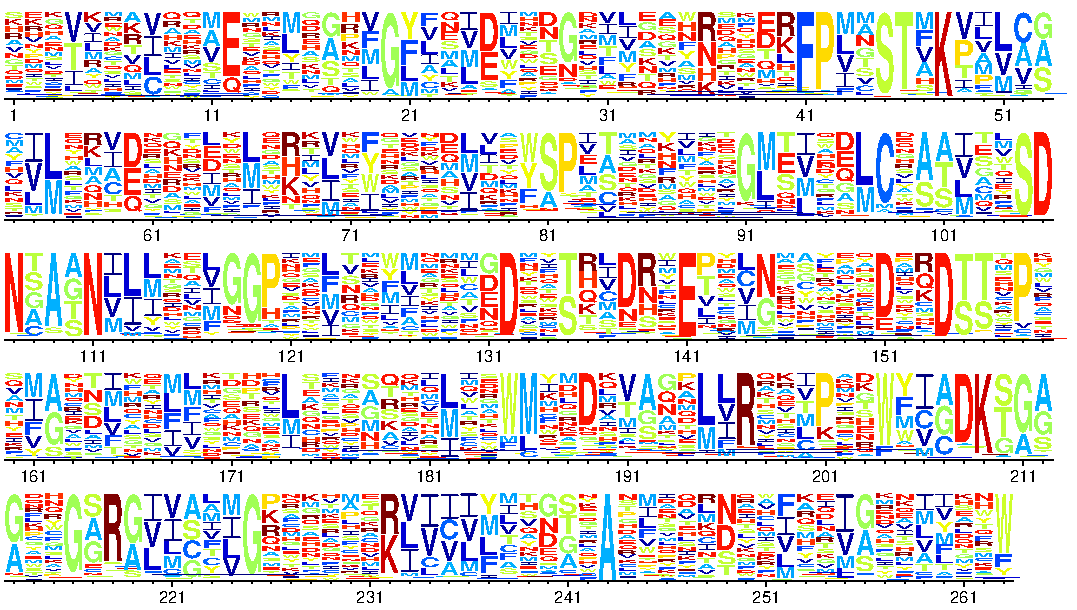
\includegraphics[width=\textwidth, page=1] {prefs_plots_lactamase_stiffler.pdf}
    \caption[Deep mutational scanning profile]{
    Site-specific deep mutational scanning data on beta-lactamase of \citet{Stiffler2015}.
    For each site, preferences of the 20 amino acids are represented by the height of the corresponding amino-acid letter.
    The analysis is performed using phydms~\citep{Hilton2017}.}
    \label{fig:intro-deep-mut-profile}
\end{figure}
Even though it is possible to compare estimated fitness profiles under phylogenetic codon models with predicted profiles under biophysical modelling, I argue that this congruence and confrontation are scarcely made.

\subsection{Structurally constrained site-interdependent codon models}
\label{subsec:structurally-constrained-site-interdependent-codon-models}

It has long been realized that inter-residue interactions within the protein conformation lead to amino-acid fixation probabilities that are dependent upon the amino acid present at other sites.
More generally, site-specific fixation probabilities may change along an evolutionary trajectory because the selection coefficient of a given mutation may depend on the specific sequence background in which it occurs~\citep{Goldstein2016}.
However, either classical codon models or mechanistic codon models rely on the assumption of site independence, where each site of the protein is modelled as an independent Markov process.
Accordingly, each site is considered separately, and defines an independent Markov substitution process along the branches of a tree.

From a modelling and inference perspective, accounting for epistasis is challenging both in terms of parametrization and computational complexity~\citep{Manhart2014}.
Means of relaxing this assumption have been pursued, usually with dependence introduced between a limited number of sites~\citep{Felsenstein1996}.
In particular, models explicitly treating protein structure and site interdependencies have been developed, recruiting a coarse-grained protein structure conjointly to a statistical potential scoring the compatibility between sequence and structure, in order to evaluate the probability of fixation of a given mutation~\citep{Robinson2003, Rodrigue2005}.

Subsequently, methods to assess the statistical fit of such computationally complex models had been developed~\citep{Rodrigue2009}, as well as refinement of statistical potentials~\citep{Kleinman2010}.
These structurally constrained models have been shown to fit data better than the corresponding models that ignore protein structure.
However, some of the available site-specific phylogenetic codon models still better fit to the data than structurally constrained models, possibly indicating that alternative models should be explored in order to better incorporate structural constrain and protein biophysics.

Alternatively, assumption of site independence can be understood as considering that substitution process at the level of sites are averaged over time, where the dependencies to other sites are integrated over the course of the process.
As a result, statistical method relying on site-specific processes while accounting for epistasis consists in obtaining the marginal process for a specific site, derived analytically from the joint process integrated over the other sites.
Projecting a joint process of several sites into a single site process leverages mean-field theory developed in statistical physics, and has been used to develop phylogenetic models accounting for protein structure~\citep{Chi2018} and protein stability~\citep{Arenas2015a, Arenas2017}.
Unfortunately, these methods are not parameterized directly in terms of parameters of evolution, namely mutation and effective population size, and the estimated fitness parameters cannot be related to empirically determined parameters.

\section{General conclusions}

Finally, models of protein biophysics are appealing to evolutionary biologists since they are based on theoretical ground and can also be confronted to empirical data.
However, integration of protein biophysics models into the framework of phylogenetic inference is difficult, and inference models have to balance the trade-off between complexity and simplicity.
Moreover, I argue that phylogenetic model should be mechanistic in principle, or, in other words, they should be defined in terms of parameters that can be accessed by independent experimental means, such as to confront estimates.
As an example, analytical models of protein biophysics relating probability of fixation to molecular and thermodynamics parameters can be fitted to protein-coding \acrshort{DNA} sequences, and estimates can be compared to their empirically determined counterpart, such as to verify and solidify the soundness of both phylogenetic inference and protein biophysics.
